\chapter{Sliding Motion Planning Benchmarks}
\label{chap:app-sliding}

The motion planning algorithms presented in Chapter
\ref{chap:wholebody-planning} have been implemented using
KineoWorks\texttrademark \cite{laumond2006kcs}. The planning times
have been measured on an Intel Core~2~Duo 2.13~GHz PC with 2~GB of
RAM. Evaluation of the randomized algorithm has been conducted by
executing 500 trials on each scenario using two flavors of RRT: the
classic RRT and IPP-RRT \cite{FERR04A}. We present the results in
Figures \ref{fig:rrt-it}, \ref{fig:rrt-t} and \ref{fig:rrt-n}.

\begin{figure}[h]
\centering
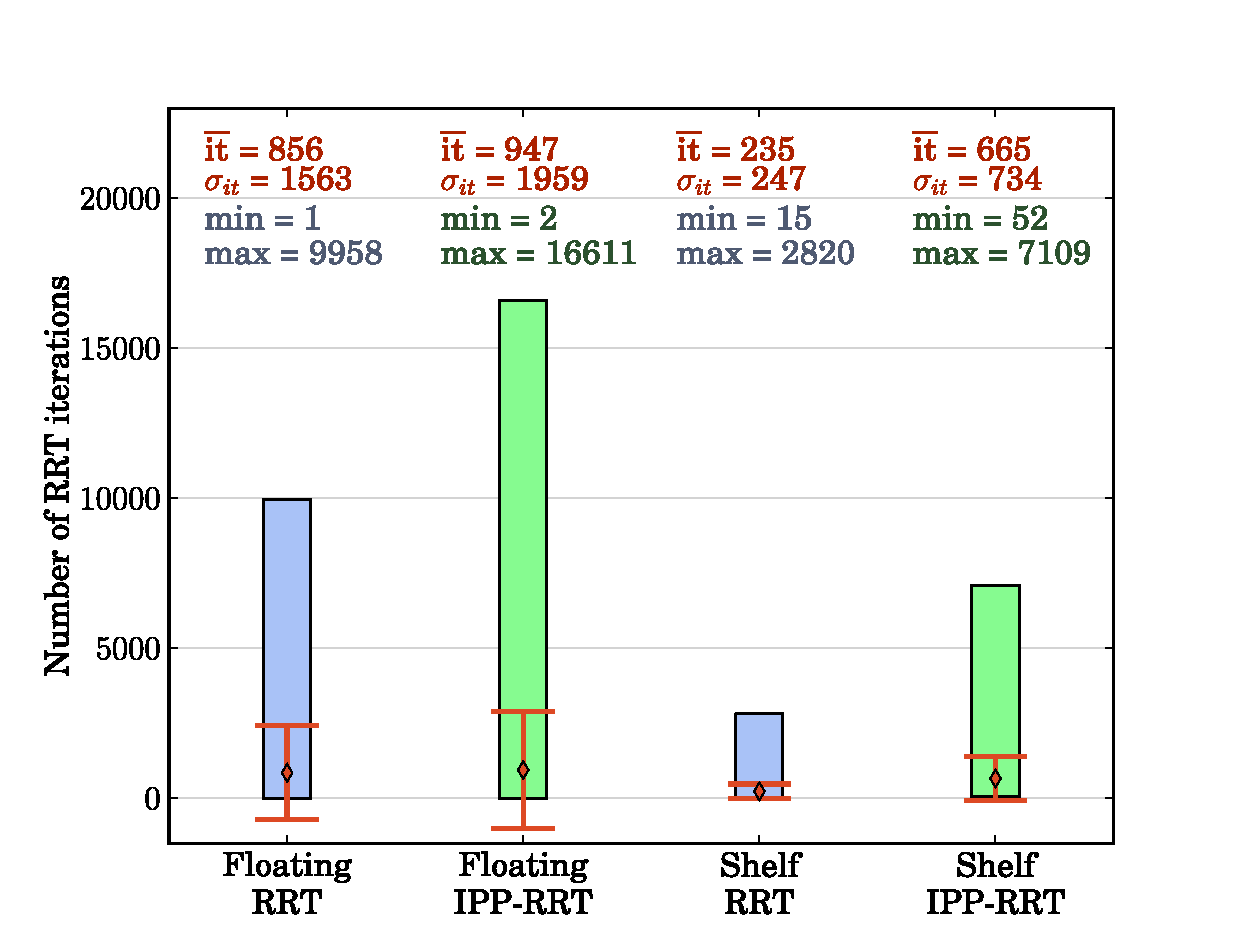
\includegraphics[width=0.7\linewidth]
                {src/appendix/plots/rrt-it.eps}
\caption{Number of RRT iterations $it$ for the floating objects and the
  shelf scenarios, using two variants of RRT. Mean $\overline{it}$,
  standard deviation $\sigma_{it}$, minimum and maximum values are
  represented.}
\label{fig:rrt-it}
\end{figure}

\begin{figure}
\centering
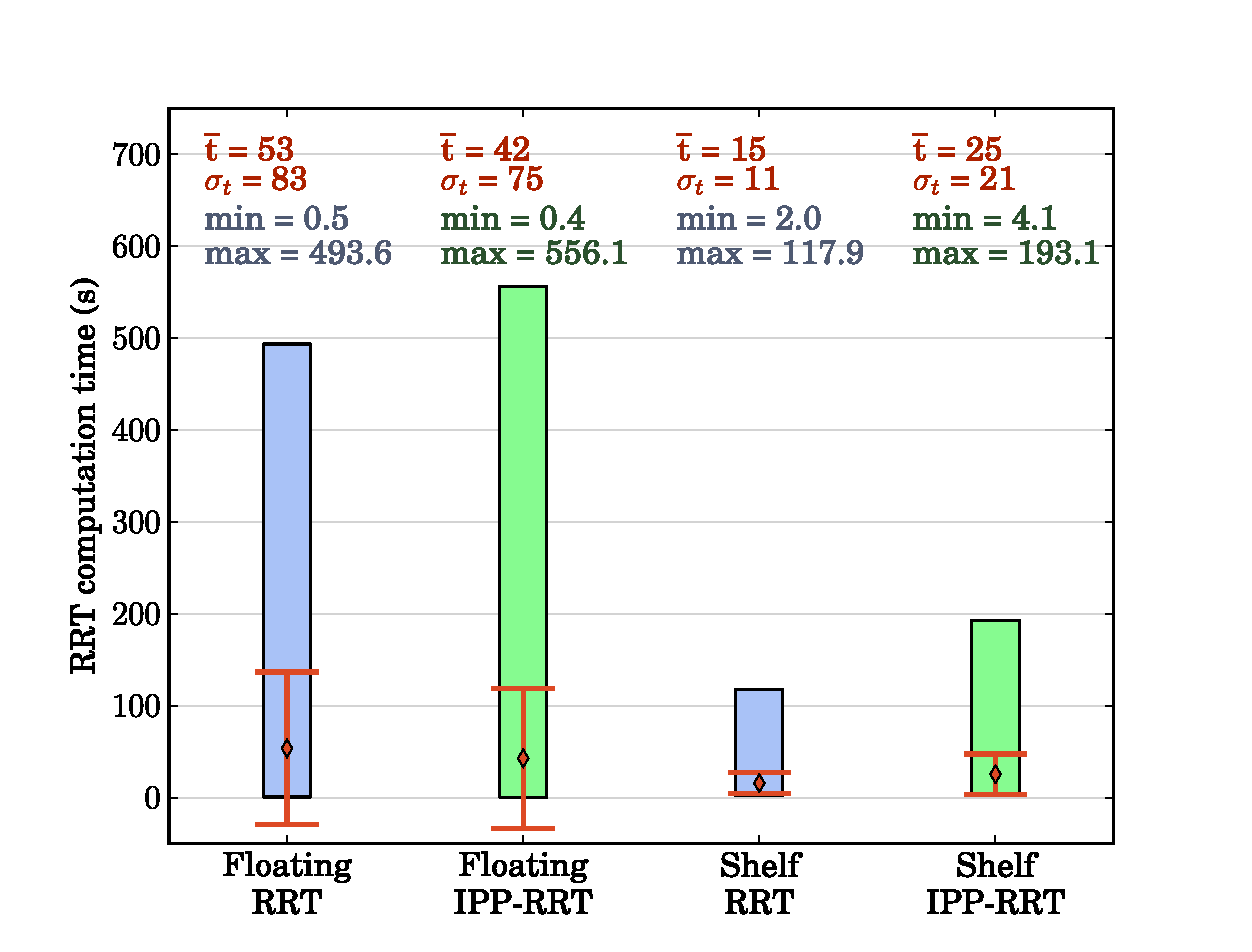
\includegraphics[width=0.7\linewidth]
                {src/appendix/plots/rrt-t.eps}
\caption{RRT computation time $t$ for the floating objects and the shelf
  scenarios, using two variants of RRT. Mean $\overline{t}$, standard
  deviation $\sigma_{t}$, minimum and maximum values are represented.}
\label{fig:rrt-t}
\end{figure}

\begin{figure}
\centering
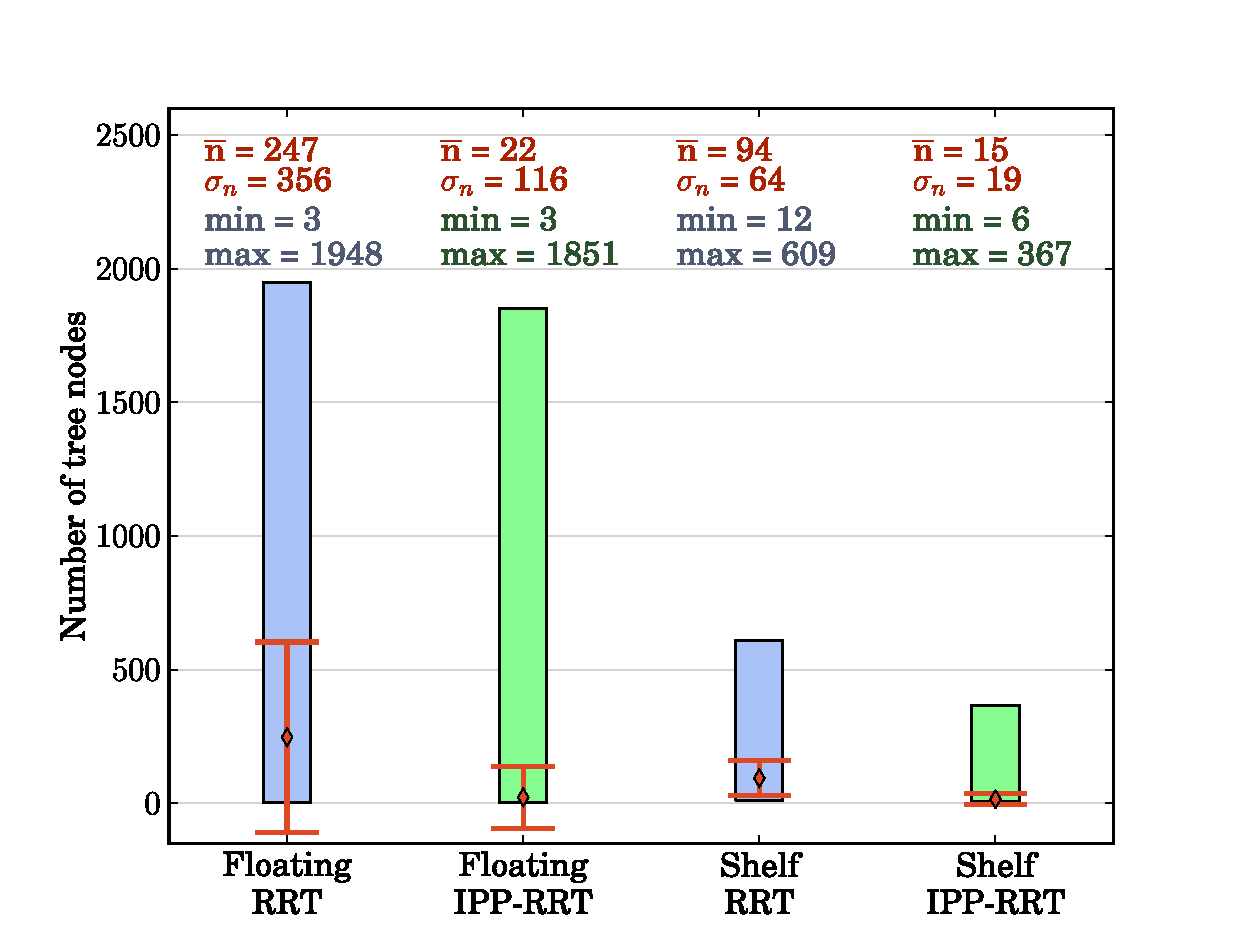
\includegraphics[width=0.7\linewidth]
                {src/appendix/plots/rrt-n.eps}
\caption{Number of tree nodes $n$ for the floating objects and the
  shelf scenarios, using two variants of RRT. Mean $\overline{n}$,
  standard deviation $\sigma_{n}$, minimum and maximum values are
  represented.}
\label{fig:rrt-n}
\end{figure}
